\section{Technical choices}

The application code is organized in two parts:

\begin{itemize}
\item A minimalist Node.js server, located in the \verb|server/| directory.
	It is statically serving the content of \verb|server/dist/|
    with compression.
\item A complete Elm client application, located in the \verb|client/| directory.
    Elm~\cite{czaplicki2013asynchronous,czaplicki2017elm}
    isn't a JavaScript framework, it is a functional programming language,
	compiling to JavaScript to run in browsers.
	Its syntax is inherited from Haskell but far simpler.
	The compiled application is 150 KB gzipped,
    which is great for low bandwidth connections.
\end{itemize}


\subsection{The application architecture}

\begin{figure}[ht]
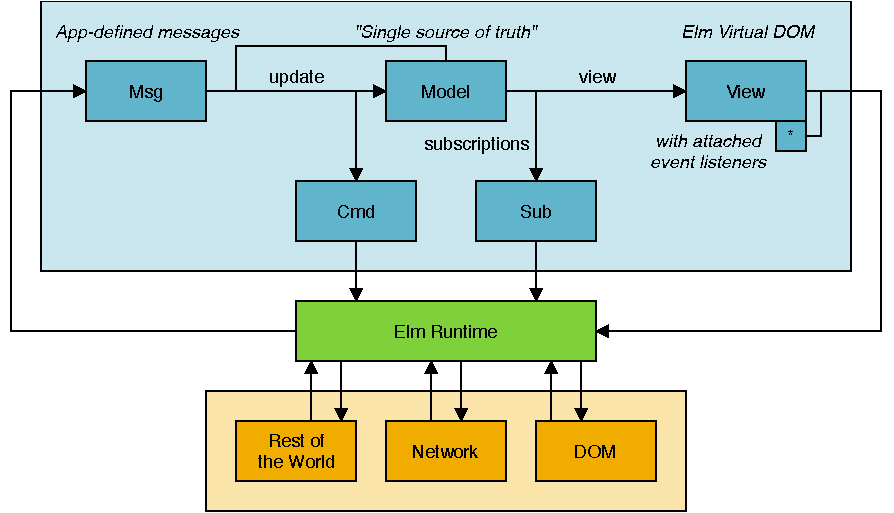
\includegraphics[width=\columnwidth]{img/tea-draw-io.pdf}
\caption{The application architecture.}%
\label{fig:tea}
\end{figure}

The application architecture enforces a unidirectional data transformation flow,
visualized in Figure~\ref{fig:tea}.
The central entity is the \verb|Model|.
It contains all and every information about our application state.
The visual aspect of our application is called the \verb|View|
(basically an HTML rendered document) which is generated by the \verb|view| function,
from the \verb|Model|. Finally, all events generate messages, of type \verb|Msg|.
The \verb|update| function, updates the model by reacting to those messages, closing the loop.

All functions are pure, meaning there is no side effect,
outputs of functions are entirely defined by inputs.
There cannot be global variables mutations,
real world events, network interaction etc.
Basically such a program would be running in a predestined way
from its start to its end,
preventing us from loading images and interacting with them.
This is why the application is attached to the Elm runtime,
provided by the language, transforming all real world events (``side effects'')
into our defined set of messages, of type \verb|Msg|.

The main challenge with pure functions is
to describe side effects without performing them.
Those are described in three locations:

\begin{enumerate}
\item View attributes as DOM event listeners for pointer events.
\item Commands (\verb|Cmd|) generated by the update function, like loading of images.
\item Subscriptions (\verb|Sub|) to outside world events like the window resizing.
\end{enumerate}

The Elm runtime takes those side effect descriptions,
perform them, and, whenever there is a result / an answer,
transforms it into one of our defined messages (\verb|Msg|)
and routes it to our update function.


\subsection{The model states}

The \verb|state| is the main component of the \verb|Model|.
It contains the images and configuration loaded as well as the annotations performed.
Its type is defined as in Listing~\ref{lst:state}
and can be modeled as a finite state machine, visualized in Figure~\ref{fig:states}.

\lstinputlisting[language=haskell,caption={State type definition.},label={lst:state},float]{code/State.txt}

\begin{figure}[ht]
\centering
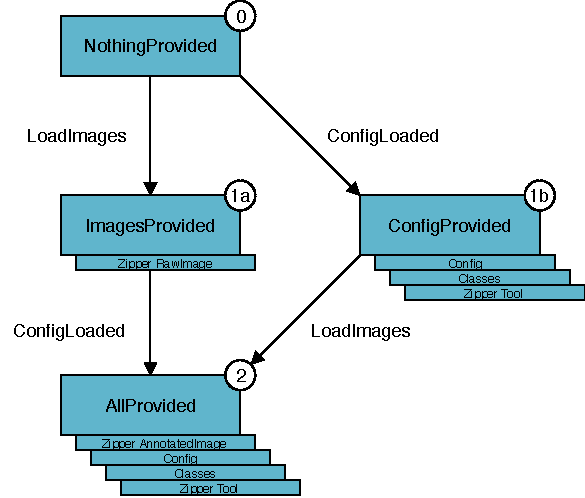
\includegraphics[width=\columnwidth]{img/states-draw-io.pdf}
\caption{The application states.}%
\label{fig:states}
\end{figure}

The application available online starts in state 0 (\verb|NothingProvided|)
and enables you to reach state 2 (\verb|AllProvided|)
with buttons to load images and configuration.
Two messages called \verb|LoadImages| and \verb|ConfigLoaded| produce
transitions in the state machine.


\subsection{The messages}

All modifications of the model are understood
by looking at the \verb|Msg| type definition (Listing~\ref{lst:msg}).
The \verb|update| function then performs the modifications described by those messages.

\lstinputlisting[language=haskell,caption={Msg type definition.},label={lst:msg},float]{code/Msg.txt}

\begin{itemize}
\item The \verb|WindowResizes| message is triggered when the application is resized.
	In the update function, it takes the new size and recomputes some view parameters.
\item A \verb|PointerMsg| message is triggered by pointer events (mouse, touch, etc.).
	In the update function, this is the message activating
	all the annotations logic code of our application.
\item The messages \verb|SelectImage|, \verb|SelectTool| and \verb|SelectClass|
	are generated when clicking on images, tools and classes.
\item Files are handled by five messages:
	\begin{itemize}
	\item When selecting images in the file explorer to load,
		a \verb|LoadImages| message is generated with a list of the images files
		and their names as identifiers.
		For each image correctly loaded an \verb|ImageLoaded| message is generated,
		providing a local url, corresponding to the image in memory.
    \item The messages \verb|LoadConfig| and \verb|ConfigLoaded| behave similarly.
    \item The \verb|Export| message causes the application to serialize into JSON
		all the annotations, and asks the user to save the generated file.
		It is triggered by clicking on the export button of the top action bar.
	\end{itemize}
\item Whenever an event should change the zooming level of the drawing area,
	a \verb|ZoomMsg| message is  generated.
\item Finally, the \verb|RemoveLatestAnnotation| message is also explicit.
\end{itemize}


\subsection{The view}

The view of this application is based on four components,
each implemented in its own module, with potentially different versions
depending on the current state of the application.
\begin{itemize}
\item The top action bar (\verb|src/View/ActionBar.elm|).
\item The center annotations viewer area\\(\verb|src/View/AnnotationsArea.elm|).
\item The right images sidebar\\(\verb|src/View/DatasetSideBar.elm|).
\item The left classes sidebar\\(\verb|src/View/ClassesSideBar.elm|).
\end{itemize}


% \subsection{Startup and interactions with JavaScript}

% Compiling the Elm application code produces a JavaScript file \verb|Main.js|.
% This file has to be embeded in an html document.
% Then the application is started with parameters called "flags"
% as demonstrated in Listing~\ref{lst:start}.

% \lstinputlisting[language=javascript,caption={JavaScript code to embed the Elm application.},label={lst:start},float]{code/start.js}


\subsection{Library and application duality}

In order to offer a turnkey solution to image annotations,
we created a configurable application solving most needs.
But we also thought of cases where advanced modifications are required.
Consequently, the foundation of this application has been extracted
in the independent package elm-image-annotation~\cite{annotationpackage}.
It is designed as an API to create, modify and visualize geometric shapes,
useful in the context of image annotation.

Modules for manipulation and serialization (in JSON) of annotations are
under the \verb|Annotation.Geometry| namespace.
It already contains one module for each tool presented earlier.
If you want to introduce a new tool, this is where you can create a new module.

This package also contains the following important modules,
under the \verb|Annotation| namespace:
\begin{itemize}
	\item \verb|Annotation.Style|:
		defines types describing appearance of points, lines and fillings of annotations.
	\item \verb|Annotation.Svg|:
		exposes functions rendering SVG elements for each annotation kind.
	\item \verb|Annotation.Viewer|:
		manages the central visualization area,
		supporting zooming and translations, relative to an image frame.
\end{itemize}
If you are interested in creating another rendering target than SVG,
like canvas, WebGL, \ldots, it would require alternative modules
to \verb|Annotation.Svg| and \verb|Annotation.Viewer|.
The rest of the code can stay unchanged.
